\documentclass{article}

\setlength{\topmargin}{-.5in}
\setlength{\oddsidemargin}{.125in}
\setlength{\textwidth}{6.25in}

% page numbering style
\usepackage{fancyhdr}
\pagestyle{fancy}
\renewcommand{\headrulewidth}{0pt}
\fancyhf{}
\fancyfoot[R]{\thepage}
\fancypagestyle{plain}{%
    \renewcommand{\headrulewidth}{0pt}%
    \fancyhf{}%
    \fancyfoot[R]{\thepage}%
}

\usepackage{float}

\usepackage{Sweave}
\begin{document}
\Sconcordance{concordance:report.tex:report.Rnw:%
1 20 1 1 0 2 1 1 12 1 4 1 25 23 1 1 19 2 1 2 2 342 1 1 43 2 1 2 2 2 1 1 %
34 1 22 1 3 4 0 1 2 1 1}





\title{Mathematics Developers Survey 2016}
\author{Nejc Ilenic}
\date{}
\maketitle

\section{Introduction}
Anonymised responses from Stack Overflow Annual Developer Survey are published each year along the results to encourage their further analysis. Being curious about where in the world and in which domain a data scientist should start his / her career, we attempt to answer some of the relevant questions by analysing the available dataset.

\vspace{2mm}

An important thing to note when interpreting the results however is that this data may not be a represantative sample from the population of mathematics developers. One should keep in mind that these are developers who were aware of the survey and were willing to answer the questions.

\section{Data preparation}
The dataset was constructed from survey that took place from January 7 to January 25, 2016, with responses originating from Stack Overflow, Stack Exchange technical sites, Facebook and Twitter. Most of the questions are demographic or relating to professional work and technology. Raw data consists of 56030 samples and 66 features, all of which are optional.

In order to obtain an adequately sizable sample, we have decided to include all respondents that belong to the occupation group of mathematics developers, which includes data scientists, machine learning developers and developers with statistics and mathematics backgrounds. After filtering out other occupations and responses with unknown countries there are 2132 samples left for the analysis.

\section{Exploratory analysis}
We are primarily interested in answering two questions: where in the world and in which domains (industries) are mathematics developers satisfied with their jobs the most. Additionally, we want to learn how job satisfaction depends on other factors like compensation, age, gender, etc. We will attempt to answer the first two questions by comparing the level of satisfaction across groups and the last one by estimating linear relationships between variables.

\subsection{Job satisfaction among countries}
Number of mathematics developers per countries can be seen in Figure \ref{fig_0}. Minimum number of 35 respondents is required to take the country into account and all others are placed into a single group called \textit{Other}. Note that selected countries and number of answers may be different when doing inference of specific features due to missing values (i.e. optional answers in the survey). Majority of respondents are from United States, followed by a combination of countries with less than 40 developers, United Kingdom, Germany and India.


\begin{figure}[H]
\centering
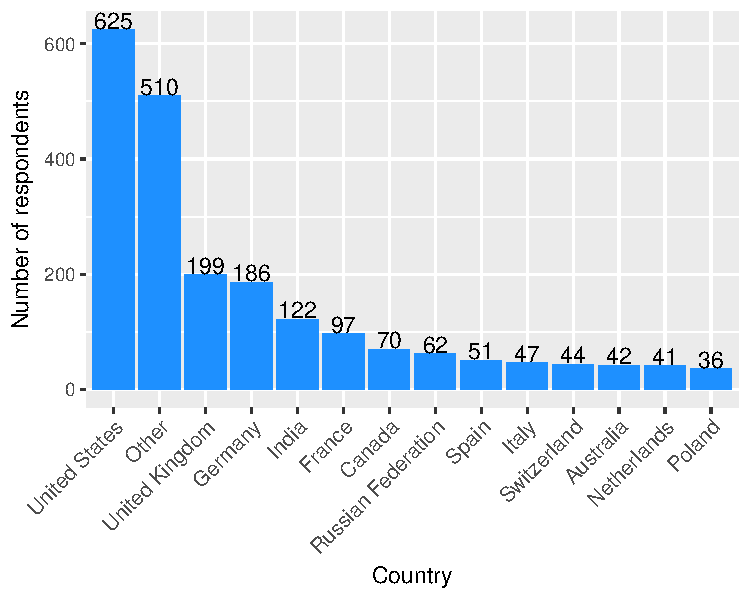
\includegraphics{report-005}
\caption{Number of mathematics developers per country.}\label{fig_0}
\end{figure}

The question from the survey regarding job satisfaction is: 'How satisfied are you with your current job(s)?' with six possible answers: 'I don't have a job', 'I hate my job', 'I'm somewhat dissatisfied with my job', 'I'm neither satisfied nor dissatisfied', 'I'm somewhat satisfied with my job' and 'I love my job'. This is a typical approach to scaling answers in survey research and we will treat the response as a categorical variable for group comparison. Additionally, we will discard answers of people without the job, resulting in five categories.

A multinomial-dirichlet model can be used to model categorical data and since we are mainly interested in a single category ('I love my job') an alternative would be to transform it to a binary variable and use a binomial-beta model instead. Nevertheless, we will model all five categories simultaneously and focus on a single category when interpreting the results. Note that both dirichlet and beta priors are conjugate for the two sampling models and posteriors could easily be derived analytically, we will still use MCMC approximations as an alternative.

A posterior parameters sample is obtained for each country independently by running a MCMC algorithm for 5000 iterations with 400 warmup samples. We have no opinions or information from related studies regarding parameters, thus uninformative priors are used. Traceplots and MCMC summaries are not included in the report, but can be found in the \textit{plots} and in the \textit{mcmc\_summaries} directories. Nothing abnormal can be spotted and it seems that all the chains have converged.

In Figure \ref{fig_1} a posterior predictive check can be seen. Sampling distributions of log odds of the answer 'I love my job' calculated from posterior predictive samples of the same sizes as the observed samples are plotted for each of the countries and there are no noticeable discrepancies between the replicated the observed data (with respect to the selected statistic). Note that visual posterior predictive checks are 'sanity checks' more than anything else (e.g. their usage as a model selection technique would be quite inadequate).





\begin{figure}[H]
\centering
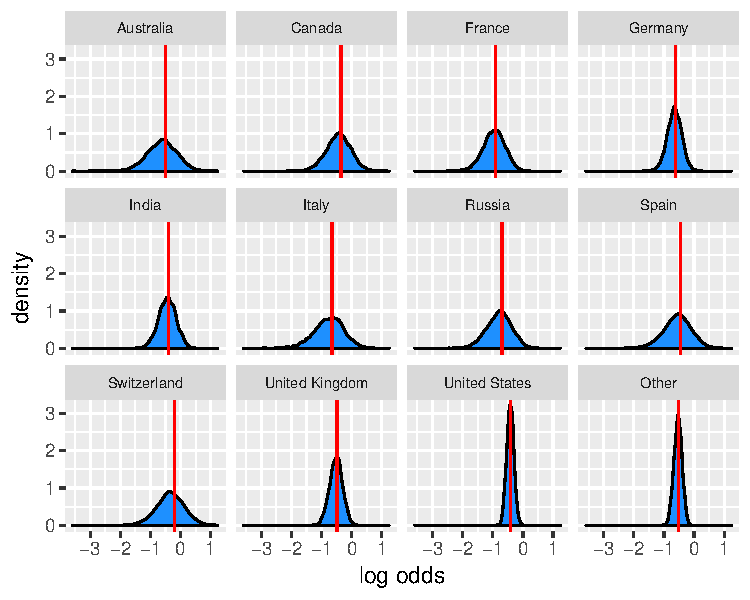
\includegraphics{report-010}
\caption{Job satisfaction between countries posterior predictive check. Densities are sampling distributions of log odds of the answer 'I love my job' calculated from posterior predictive samples of the same sizes as the observed samples. Red lines indicate the observed log odds.}\label{fig_1}
\end{figure}

Result of the sampling can be seen in Figure \ref{fig_2}. Plotted are 90\% confidence intervals for posterior probabilities of the answer 'I love my job' for all countries. It can be concluded that there are either no meaningful differences among the countries regarding the probability of someone loving his / her job or we simply can't answer the question with this data. We can however take a more indirect approach by estimating which variables are positively correlated with job satisfaction and compare those among groups instead.


\begin{figure}[H]
\centering
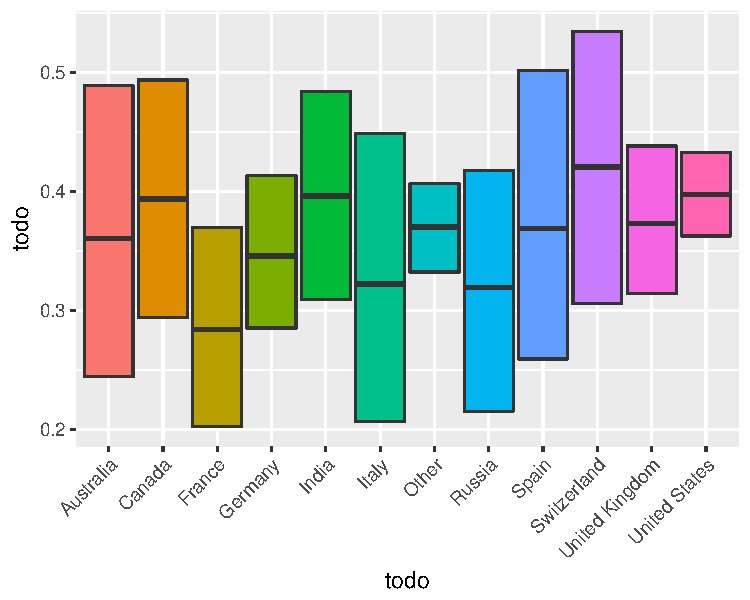
\includegraphics{report-012}
\caption{90\% confidence intervals for posterior probabilities of the answer 'I love my job' for all countries.}\label{fig_2}
\end{figure}

\subsection{Explanatory variables for job satisfaction}
Here we are concerned with how job satisfaction varies with a set of selected variables. Specifically, we are interested in how person's age, gender, purchasing power, whether he or she works remotely, values unit testing, commits code at least once a day and whether he or she works in a big company and has PhD explain the level of their job satisfaction. Age and purchasing power are continuous and all other variables are binary. It should be stated that purchasing power is calculated as compensation in dollars divided by a Big Mac index of the respondent's country (an informal way of measuring the purchasing power parity, i.e. how many Big Macs can a person buy per year) and company is regarded big if number of employees is more than 99. All other variables should be self explanatory.

We will treat the outcome (5 possible answers as before) as an ordinal variable (i.e. a categorical for which values are ordered, but the distances between them are unknown) to preserve information regarding the order. Ordinal logistic regression with uninformative priors is our model of choice here. Again 5000 posterior samples are drawn using a MCMC algorithm with 400 warmup iterations. Traceplots and MCMC summaries are not included in the report, but can be found in the \textit{plots} and in the \textit{mcmc\_summaries} directories. Nothing abnormal can be spotted and it seems that all the chains have converged.

In Figure \ref{fig_3} a posterior predictive check can be seen. Plotted are histograms of 20 replicated samples along with a histogram of the observed sample. In some plots differences can be spotted between replicated and observed data and in others histograms are almost identical. We will conclude that our model fits the data sufficiently for our purposes and assume that discrepancies are due to the sampling variability.





\begin{figure}[H]
\centering
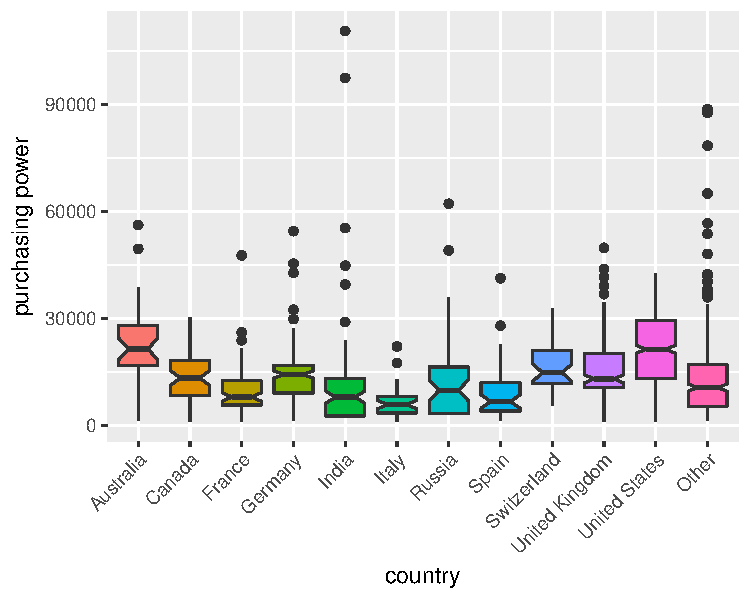
\includegraphics{report-017}
\caption{Posterior predictive check for conditional distribution of job satisfaction given explanatory variables. Plotted are histograms of 20 replicated samples along with a histogram of the observed sample.}\label{fig_3}
\end{figure}

The observed Pearson correlation coefficients (covariance of the two variables divided by the product of their standard deviations) of selected explanatory variables are plotted in Figure \ref{fig_4}. There are no strong correlations between regressors with exception of correlation between age and purchasing power ($+0.36$), which we have to keep in mind when interpreting the regression coefficients. Otherwise these results seem somewhat reasonable: remote work is positively correlated with age and negatively with working in a big company and age is positively correlated with purchasing power.


\begin{figure}[H]
\centering
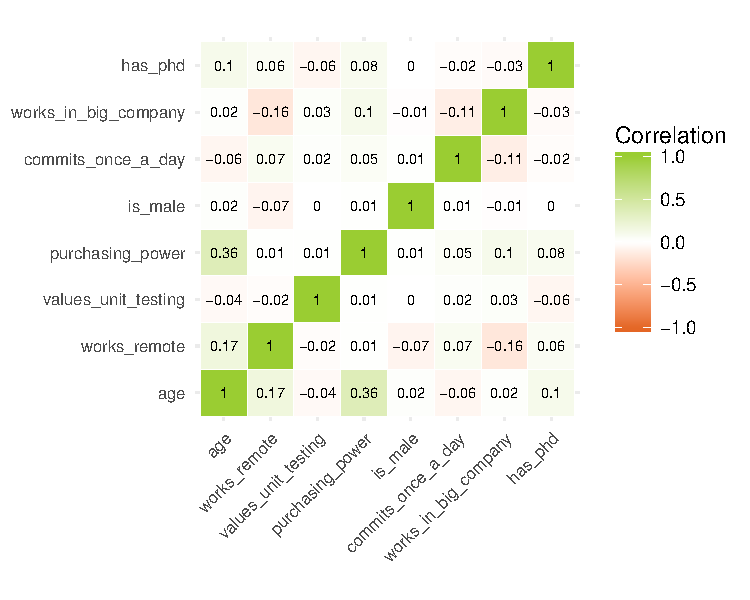
\includegraphics{report-019}
\caption{Pearson correlation coefficients of selected explanatory variables.}\label{fig_4}
\end{figure}

Next we examine posterior regression coefficients' 90\% confidence intervals in Figure \ref{fig_5}. Let's first focus on continuous variables age and purchasing power. We can't be certain but it seems that as age grows satisfaction level declines. On the other hand we can say much more confidently that purchasing power is positively correlated with job satisfaction, which seems quite reasonable. With dummy variables we have to keep in mind that we have modeled a 'reference' female developer which doesn't commit code at least once a day, doesn't have a PhD, doesn't value unit testing, doesn't work in a big company and doesn't work remotely. We can then intepret signs of coefficients as positive or negative effect that corresponding variables have if we change their values from false to true keeping all other variables constant. For example if we say that our 'reference' developer starts to work remotely it is possible that her satisfaction level will rise, although we should be conservative here as the 5th percentile is actually below zero. Similarly if she starts to work in a big company it is likely that her satisfaction level will decline. 90\% confidence intervals of other variables contain the value of zero so we won't conclude their effect on response variable. Our level of uncertainty is the lowest for purchasing power so we turn our attention to that in the next section.


\begin{figure}[H]
\centering
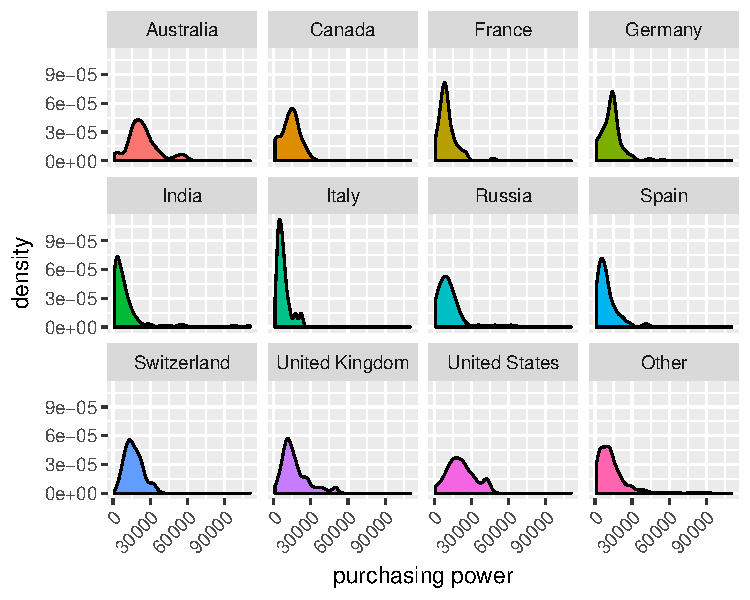
\includegraphics{report-021}
\caption{90\% confidence intervals for posterior regression coefficients of selected explanatory variables for job satisfaction.}\label{fig_5}
\end{figure}

\subsection{Purchasing power among countries}
We will compare purchasing power among countries as results in previous section strongly suggest its positive correlation with job satisfaction. In spite of that one should bear in mind that the highest purchasing power doesn't imply the highest job satisfaction and that the opposite case can occur just as well. There may be other (even unmeasured) factors that we have not taken into account and have stronger (negative) correlation with job satisfaction. The only conclusions we will be able to draw based on results from this section are regarding the purchasing power itself.

In Figure \ref{fig_6} we can see the observed densities of purchasing power for all countries. Based on the plots it seems that gamma or Weibull models would be appropriate for this random variable, however as we are only interested in comparing means across groups we can use the normal model (central limit theorem). Additionally we turn to the hierarchical normal model to combine the information from all countries.


\begin{figure}[H]
\centering
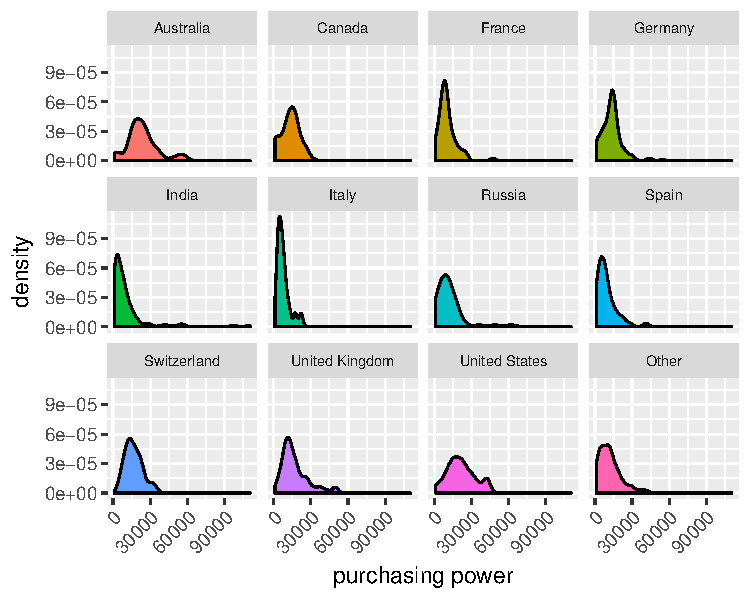
\includegraphics{report-023}
\caption{Observed densities of purchasing power for all countries.}\label{fig_6}
\end{figure}

A posterior sample of group means is obtained for each country independently by running a MCMC algorithm for 5000 iterations with 400 warmup samples. Like before we have no opinions or information from related studies regarding parameters, thus uninformative priors are used. Traceplots and MCMC summaries are not included in the report, but can be found in the \textit{plots} and in the \textit{mcmc\_summaries} directories. Nothing abnormal can be spotted and it seems that all the chains have converged.

Posterior predictive check can be seen in Figure \ref{fig_7}. Sampling distributions of means of posterior predictive samples of the same sizes as the observed samples are plotted along with the observed means. We can observe a practical demonstration of the central limit theorem (larger sample size - smaller standard error). There are no noticeable discrepancies between the replicated the observed data with respect to the selected statistic (the mean).




\begin{figure}[H]
\centering
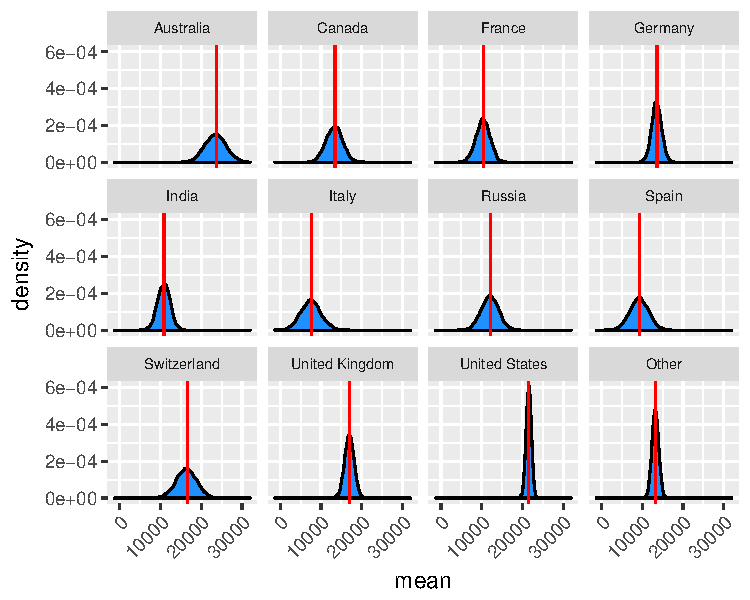
\includegraphics{report-027}
\caption{Purchasing power between countries posterior predictive check. Densities are sampling distributions of means of posterior predictive samples of the same sizes as the observed samples. Red lines indicate the observed means.}\label{fig_7}
\end{figure}

Result of the sampling can be seen in Figure \ref{fig_8}. Plotted are 90\% confidence intervals for purchasing power posterior means for all countries. We won't calculate exact probabilities of comparisons of means (although we could, we have the posterior distributions), but rather compare them visually. Mean purchasing power is higher in United States and Australia than in all other countries (more than 20000 Big Macs per year). United Kingdom has higher mean purchasing power than all other countries (excluding United States and Australia) and seems similar to Switzerland's, although level of uncertainty is much higher for the latter due to a smaller sample size. Canada, Germany and all countries with less than 35 respondents combined have higher mean purchasing power than Italy.

In next sections the same comparisons for job satisfaction and purchasing power are given for different domains (industries) rather than countries. All methodologies (models, number of iterations of a MCMC algorithm, etc) are identical to previous sections, thus only interpretations are given.


\begin{figure}[H]
\centering
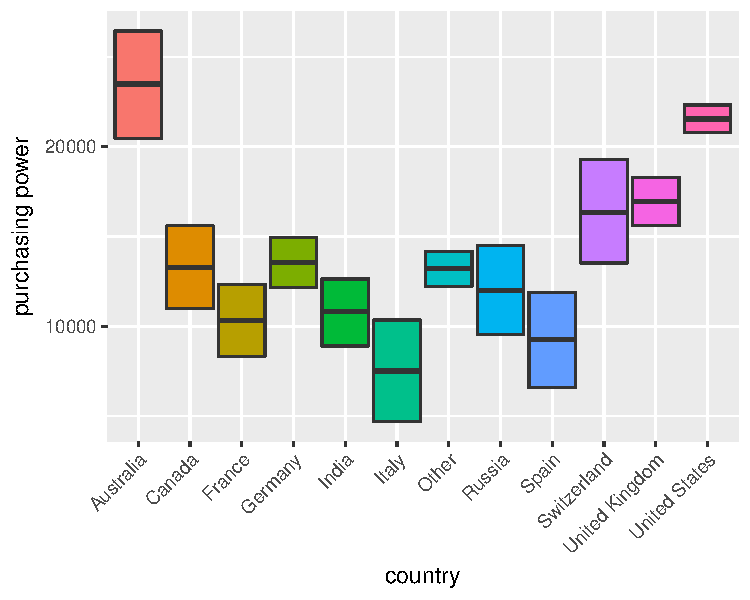
\includegraphics{report-029}
\caption{90\% confidence intervals for purchasing power posterior means for all countries.}\label{fig_8}
\end{figure}

\subsection{Job satisfaction among industries}
Number of mathematics developers per industries can be seen in Figure \ref{fig_9}. As before, minimum number of 35 respondents is required to take the industry into account and all others are placed into a single group called \textit{Other}. Note that selected industries and number of answers may be different when doing inference of specific features due to missing values (i.e. optional answers in the survey).


\begin{figure}[H]
\centering
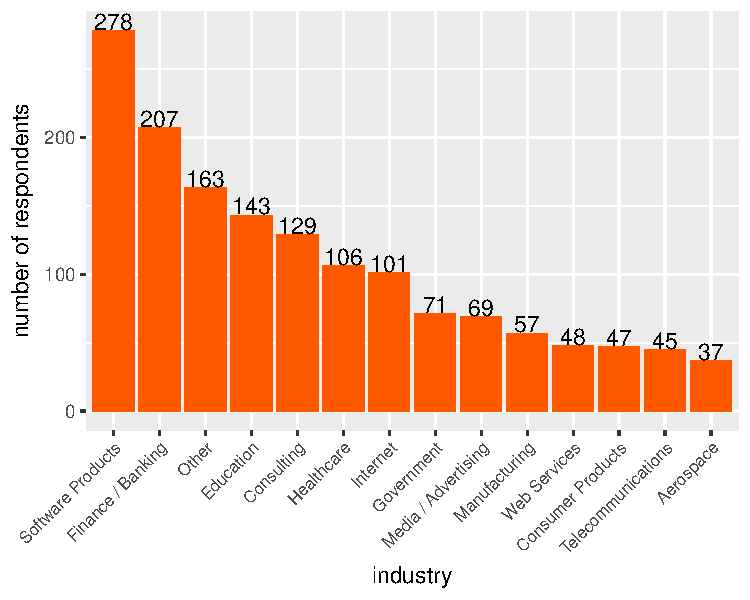
\includegraphics{report-031}
\caption{Number of mathematics developers per industry.}\label{fig_9}
\end{figure}

In Figure \ref{fig_10} a posterior predictive check can be seen. Like previously, sampling distributions of log odds of the answer 'I love my job' calculated from posterior predictive samples of the same sizes as the observed samples are plotted for each of the industries and there are no noticeable discrepancies between the replicated the observed data (with respect to the selected statistic). An interesting regard is that the log odds ratio, like the mean, also has a normal asymptotic distribution.





\begin{figure}[H]
\centering
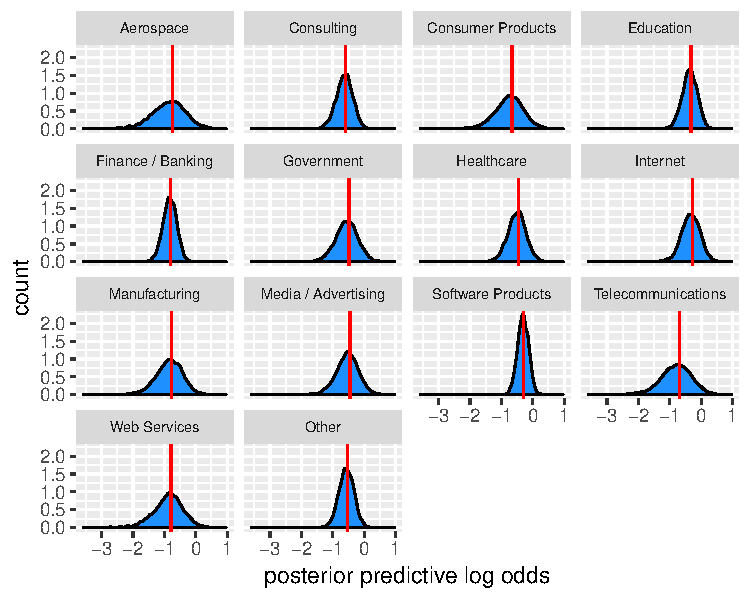
\includegraphics{report-036}
\caption{Job satisfaction between industries posterior predictive check. Densities are sampling distributions of log odds of the answer 'I love my job' calculated from posterior predictive samples of the same sizes as the observed samples. Red lines indicate the observed log odds.}\label{fig_10}
\end{figure}

Result of the sampling can be seen in Figure \ref{fig_11}. Plotted are 90\% confidence intervals for posterior probabilities of the answer 'I love my job' for all industries. The only speculations we can make with this data is that for the Software Products and Education domains the probability of the answer 'I love my job' seems higher than for the Finance / Banking domain (although we will stay conservative and not make any conclusions).


\begin{figure}[H]
\centering
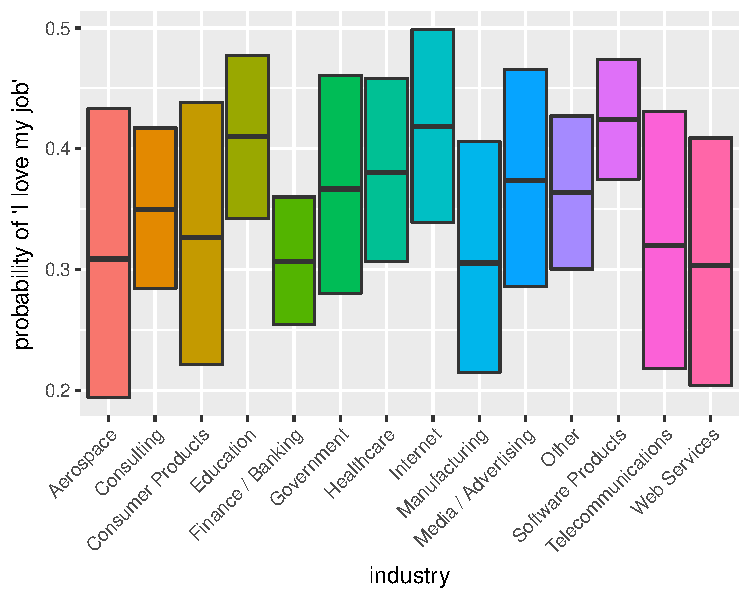
\includegraphics{report-038}
\caption{90\% confidence intervals for posterior probabilities of the answer 'I love my job' for all industries.}\label{fig_11}
\end{figure}

\subsection{Purchasing power among industries}
In Figure \ref{fig_12} the observed densities of purchasing power for all industries can be seen. The gamma or Weibull distributions could again be used as our first attempts at modeling if we wouldn't only be interested in the mean.


\begin{figure}[H]
\centering
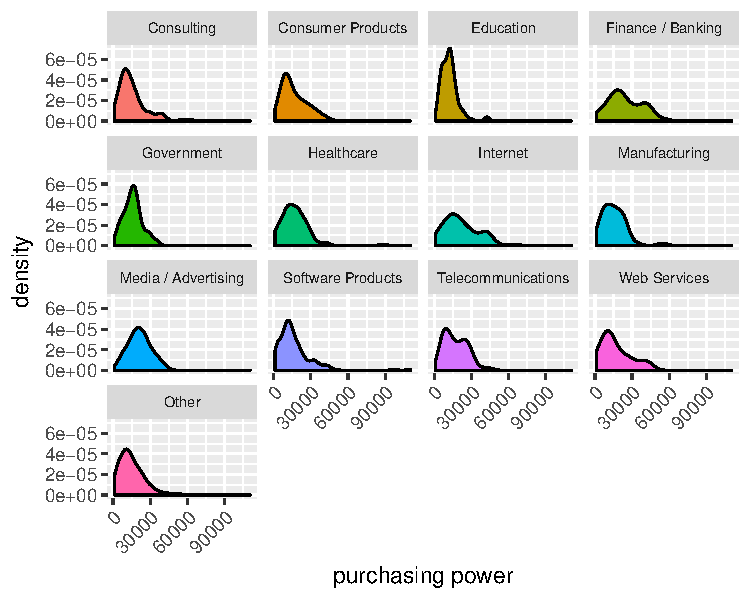
\includegraphics{report-040}
\caption{Observed densities of purchasing power for all industries.}\label{fig_12}
\end{figure}

Posterior predictive check can be seen in Figure \ref{fig_13}. Sampling distributions of means of posterior predictive samples of the same sizes as the observed samples are plotted along with the observed means. There are no noticeable discrepancies between the replicated the observed data with respect to the selected statistic (the mean).




\begin{figure}[H]
\centering
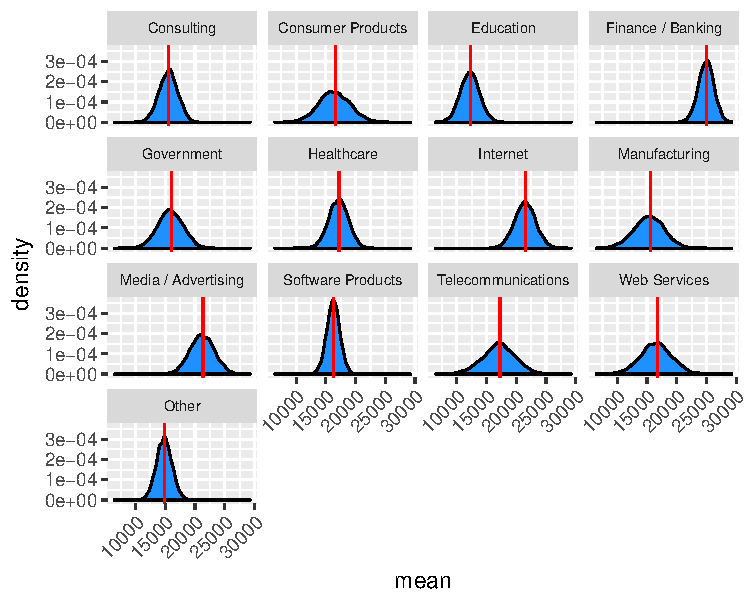
\includegraphics{report-044}
\caption{Purchasing power between industries posterior predictive check. Densities are sampling distributions of means of posterior predictive samples of the same sizes as the observed samples. Red lines indicate the observed means.}\label{fig_13}
\end{figure}

Result of the sampling can be seen in Figure \ref{fig_14}. Plotted are 90\% confidence intervals for purchasing power posterior means for all industries. We are most certain that the mean purchasing power is higher in Finance / Banking than in all other domains (except in the Internet domain and the Media / Advertising domain). Mathematics developers in Education have lower mean purchasing power than those in the Software Products, Media / Advertising, Internet, Healthcare and Finance / Banking domains.


\begin{figure}[H]
\centering
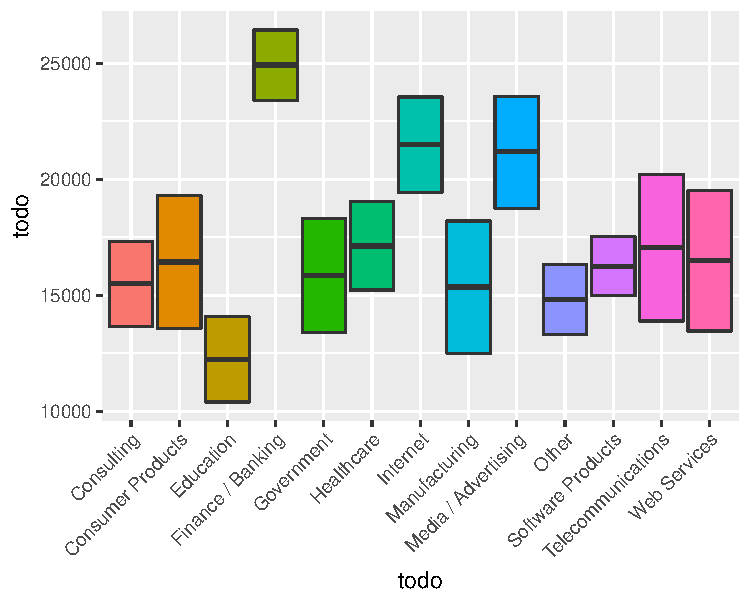
\includegraphics{report-046}
\caption{90\% confidence intervals for purchasing power posterior means for all industries.}\label{fig_14}
\end{figure}

\section{Conclusion}
In this project we compared probabilities that a mathematics developer loves his / her job and mean purchasing powers among countries and industries. Additionally, we were interested in how job satisfaction varies with a set of selected variables.

We suspect that age and working in a big company is negatively correlated with job satisfaction, we suspect that working remotely is positively correlated with job satisfaction and we are quite certain that purchasing power is positively correlated with job satisfaction. Our degree of belief is quite high that mean purchasing power is the highest in Australia and United States. We also believe, that mean purchasing power is the highest in the Finance / Banking industry.

\end{document}
